% ============================================================
% 片段：s06  对应原文 appendix1.tex 第 1--105 行；PDF 第 66--68 页
% 内容：附录 A  Čech 上同调
% 译者：lead   审校状态：初稿
% ============================================================

% ==== 原文 PDF 第 66 页 ====
\section{Čech 上同调}

\begin{keytakeaways}
  \begin{itemize}[leftmargin=1.4em,itemsep=2pt,topsep=2pt]
    \item \textbf{物理图像}：Čech 上同调把“如何在流形上一致地给连线赋群元素”这一物理问题（平坦联络、和乐）翻译成纯组合数据：坐标卡是 0-单纯形、交集是 1-单纯形、多重交集是高维单纯形。
    \item \textbf{数学工具}：良覆盖、单纯形、边缘算子 $\ptl$、链复形；以及由预层、限制映射 $\mathrm{Res}$ 与上边缘 $\delta$ 构成的 Čech 上链复形。
    \item \textbf{关键结论}：物理上关心的平坦联络局部数据满足 $A_{ij}A_{jk}A_{ki}=\mathrm{id}$ 之类的上闭链条件，而“不一致性”（如离散挠类）正是由 $H^k(\mathcal{U},\mathcal{F})$ 的非平凡类刻画。这为正文第 2.4 节的“平坦联络”视角提供了严格框架，也是后文 2-群背景场的 twisted/shifted 上闭链条件的语言基础。
  \end{itemize}
\end{keytakeaways}

\label{App:Cech}

本附录说明如何建立一种方法，把群元素妥善地赋给流形中的连线，即如平坦联络（见第~\ref{para:flatconn}~段）所描述的那样。

在流形的构造中，大家熟知的做法是用局部欧氏空间 $\bbR^n$ 的坐标卡（patch）之并来描述流形 $M$，
并用一组跃迁函数 $f_{ij} : \phi_i(U_i\cap U_j)\to \phi_j(U_i\cap U_j)$ 把它们粘合起来。
下面我们选取一个良覆盖（good cover），其中所有交集 $U_{ij}$ 都是单连通的，且同构于 $\bbR^n$。

Čech（上）同调本质上是一种借用坐标卡交集来定义（上）同调的方法。其构造如下：
\begin{enumerate}
    \item 每个 $U_i$ 代表一个 0-单纯形；
    \item 每个 $U_{ij} \equiv U_i\cap U_j$ 代表一个 1-单纯形；
    \item 每个 $k$-单纯形表示为
    \be 
    U_{i_0,\cdots , i_k} \equiv \bigcap_{m = 0}^k U_{i_m} \ ,
    \ee
    可用图表示为
    \begin{center}
        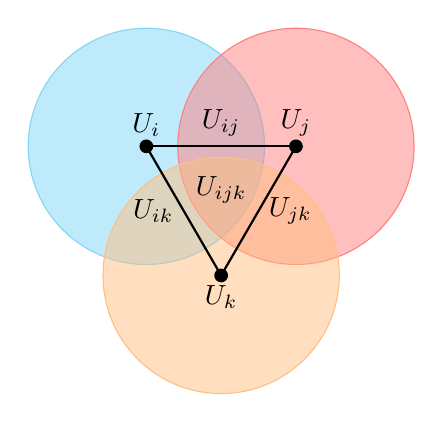
\begin{tikzpicture}
            \filldraw[ cyan!50,fill opacity=0.5 ] (0,0) circle (1.5) ; 
            \filldraw[] (0,0) circle (0.08);
            \filldraw[ red!50,fill opacity=0.5 ] (1.9,0) circle (1.5);
            \filldraw[] (1.9,0) circle (0.08);
            \filldraw[ orange!50,fill opacity=0.5 ] (0.95,-1.64) circle (1.5);
            \filldraw[] (0.95,-1.64) circle (0.08);

            \draw[thick]  (0,0)--(1.9,0)  ;
            \draw[thick]  (0.95,-1.64)--(1.9,0)   (1.425,-0.82)node[right]{$U_{jk}$};
            \draw[thick]  (0,0)--(0.95,-1.64)  (0.475, -0.82)node[left]{$U_{ik}$};
            \node[above] at (0,0) {$U_i$};
            \node[above] at (01.9,0) {$U_j$};
            \node[below] at (0.95,-1.64) {$U_k$};
            \node[above] at (0.95,0) {$U_{ij}$};
            \node[] at (0.95, -0.55) {$U_{ijk}$};
        \end{tikzpicture}
    \end{center}
    \item 边缘算子定义为\footnote{数学家可能会问加法结构从何而来。我们的说法是：现在工作在一个由 $U_{i_1,\cdots,i_k}$ 自由生成、系数取在 $\bbZ$ 中的阿贝尔群上（取其他阿贝尔群亦可）。}
    \be
    \ptl U_{i_0,\cdots ,i_k} = \sum_{m=0}^k (-1)^m U_{i_0,\cdots , \Hat{i}_m ,\cdots , i_k }
    \ee
    例如
    \be  \ptl U_{ijk} = U_{jk} -U_{ik} + U_{ij}  \ee
    图形上为
    \begin{center}
        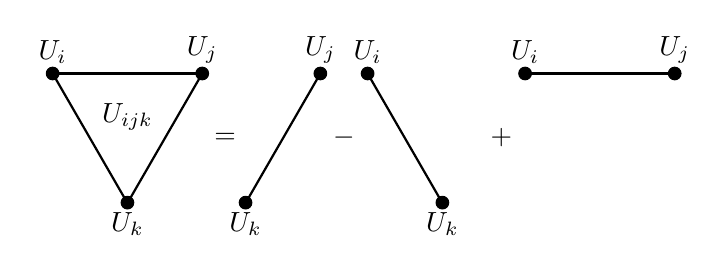
\begin{tikzpicture}
            \filldraw[] (0,0) circle (0.08);
            \filldraw[] (1.9,0) circle (0.08);
            \filldraw[] (0.95,-1.64) circle (0.08);

            \draw[thick] (0,0)--(1.9,0);
            \draw[thick,rotate = -60] (0,0)--(1.9,0);
            \draw[thick,rotate around = {60:(1.9,0)}] (1.9,0)--(0,0);
            \node[above] at (0,0) {$U_i$};
            \node[above] at (01.9,0) {$U_j$};
            \node[below] at (0.95,-1.64) {$U_k$};
            \node[] at (0.95, -0.55) {$U_{ijk}$};
            \node[] at (-0.2, -0.82){$\ptl$};
            \node[right] at (1.93, -0.82){$=$};


            
            \draw[shift = {(1.5,0)},thick,rotate around = {60:(1.9,0)}] (1.9,0)--(0,0);
            \draw[shift = {(4,0)},thick,rotate = -60] (0,0)--(1.9,0);
            \draw[shift = {(6,0)},thick] (0,0)--(1.9,0);
            \node[shift = {(4,0)},above] at (0,0) {$U_i$};
            \node[shift = {(6,0)},above] at (0,0) {$U_i$};

            \node[shift = {(1.5,0)},above] at (01.9,0) {$U_j$};
            \node[shift = {(6,0)},above] at (01.9,0) {$U_j$};

            \node[shift = {(4,0)},below] at (0.95,-1.64) {$U_k$};
            \node[shift = {(1.5,0)},below] at (0.95,-1.64) {$U_k$};
            \node[] at (3.7,-0.82) {$-$};
            \node[] at (5.7,-0.82) {$+$};

            \filldraw[shift = {(4,0)}] (0,0) circle (0.08);
            \filldraw[shift = {(1.5,0)}] (1.9,0) circle (0.08);
            \filldraw[shift = {(1.5,0)}] (0.95,-1.64) circle (0.08);
            \filldraw[shift = {(6,0)}] (0,0) circle (0.08);
            \filldraw[shift = {(6,0)}] (1.9,0) circle (0.08);
            \filldraw[shift = {(4,0)}] (0.95,-1.64) circle (0.08);

        \end{tikzpicture}
    \end{center}
    \item 容易验证，借助 $\ptl$ 算子我们得到一个 $\bbZ$-分次的链复形。记
    \be C_k(\mathcal{U}) = \bigoplus_{i_0 < i_1 < \cdots < i_k} \mathbb{Z}[U_{i_0} \cap \cdots \cap U_{i_k}] \ .  \ee
\end{enumerate}

以上是同调部分；我们更关心的是上同调部分——其中流形 $M$ 被映到各种系数中，成为我们珍视的场。我们希望场位形满足哪些性质呢？
\begin{enumerate}
    \item 场（至少是局部的）是截面 $\Gamma (U,F)$，其中 $F$ 是我们选定的某个参数空间。
    \item 为使截面映射既抽象又符合直觉，对 $V\subseteq U$ 应当存在限制映射 ${\rm Res}_{U,V} : \Gamma(U,F)\to \Gamma(V,F)$，使得
    \be  {\rm Res}_{U,U} = {\rm id}_{F} \ , \ \ \ {\rm Res}_{V,W} \circ {\rm Res}_{U,V} = {\rm Res}_{U,W} \ . \ee
    \item 对某些场，我们希望它们至少能在同一局部坐标卡上相加，即对每个 $U_i$，$\Gamma(U_i,F)$ 是一个阿贝尔群。
    于是限制映射至少应当尊重加法结构，使每个 ${\rm Res}_{U,V}$ 都是阿贝尔群同态：
    \be  {\rm Res}_{U,V} : {\rm Hom}_{\rm Ab} (\Gamma(U,F),\Gamma(V,F))  \ee
\end{enumerate}
上述语言概括起来就是：\textbf{我们想要的是 $M$ 上的阿贝尔群预层}，这种预层记作 $\mathcal{F}$。
于是，我们通过把每个 $p$-单纯形映为该单纯形上预层的一个元素，来定义一个 Čech $p$-上链 $C^p(M,\mathcal{U})$（$\CU$ 表示图册之集），即
\be
f : U_{i_1,\cdots, i_p} \mapsto G\in \CF ({U_{i_1,\cdots, i_p}})  
\ee
而微分算子 $\delta_p$ 由 ${\rm Res}$ 与 $\ptl$ 实现：对 $p$-上链，
\be
(\delta_p f)(\sigma ) = \sum_{k=0,p+1} (-1)^{k}  {\rm Res}_{\ptl_k \sigma, \sigma } (f ) (\ptl_k \sigma)   \ \
\ee
其中 $\sigma\in C^p(M,\CU)$，且 $\ptl_k (U_{i_1,\cdots,i_p}) \equiv U_{i_1,\cdots, \Hat{i}_k,\cdots,i_p} $。于是 Čech 上同调群定义为
\be  
H^k(\CU,\CF) \equiv \frac{{\rm ker}(\delta_k)}{{\rm im}(\delta_{k-1}) }  \ .
\ee

\begin{yizhu}
本附录中记号有一处容易混淆：$C_k(\mathcal{U})$（下标 $k$）是链复形中的链群，而 $C^p(M,\mathcal{U})$（上标 $p$）是上链群；
两者由预层 $\mathcal{F}$ 的截面给出。核对时请注意 $\delta_p$ 的指标：$\delta_p: C^p\to C^{p+1}$，
因此上同调 $H^k=\ker\delta_k/\operatorname{im}\delta_{k-1}$ 中分子分母的指标差一。
\end{yizhu}

\begin{yizhu}
原文在边缘算子求和中写作 $\sum_{k=0,p+1}$（逗号代替了范围符号），这是排版笔误，含义应为 $k=0,\dots,p+1$ 的求和；此处照原文保留。另，
“良覆盖”一词来自代数拓扑：要求覆盖的任意有限交集或为空、或可缩，才能保证 Čech 上同调与层上同调同构（Leray 定理）。
\end{yizhu}
